\documentclass[12pt]{article}

\usepackage[margin=1in]{geometry}
\usepackage[UTF8]{ctex}
\usepackage{amsmath}
\usepackage{booktabs}
\usepackage{tabularx}
\usepackage{array}
\usepackage{graphicx}
\usepackage{float}
\usepackage{caption}
\usepackage{hyperref}
\usepackage{natbib}

\hypersetup{
  colorlinks=true,
  linkcolor=black,
  citecolor=blue,
  urlcolor=blue,
  pdftitle={The Effect of the JPY/TWD Exchange Rate on Japanese Tourist Arrivals to Taiwan},
  pdfauthor={Wu You-Yi, Yeh Yu-Chen, Chiu Wei-Zhen, Chen Shuo-Mao, Liu Meng-Hui, Shi Shao}
}

\linespread{1.12}
\setlength{\parskip}{0.45em}
\setlength{\parindent}{0pt}
\renewcommand{\arraystretch}{1.12}
\renewcommand{\tablename}{Chart}
\renewcommand{\figurename}{Graph}
\renewcommand{\refname}{References}

\begin{document}
\newcommand{\StaticAdjRtwo}{0.8805}
\newcommand{\DynamicAdjRtwo}{0.9044}
\newcommand{\StaticFstat}{59.44}
\newcommand{\DynamicFstat}{52.19}
\newcommand{\StaticFp}{$<0.001$}
\newcommand{\DynamicFp}{$<0.001$}
\newcommand{\StaticFX}{-0.991}
\newcommand{\StaticFXP}{0.079}
\newcommand{\DynamicFX}{-1.032}
\newcommand{\DynamicFXP}{0.057}
\newcommand{\LagTourist}{0.505}
\newcommand{\LagTouristP}{$<0.001$}
\newcommand{\StaticOil}{-0.260}
\newcommand{\StaticOilP}{0.057}
\newcommand{\DynamicJIPI}{0.840}
\newcommand{\DynamicJIPIP}{0.011}
\newcommand{\BGStaticP}{$<0.001$}
\newcommand{\BGDynamicP}{$<0.001$}
\newcommand{\MaxVIFStatic}{3.27}
\newcommand{\MaxVIFDynamic}{9.75}


\begin{center}
{\LARGE \textbf{The Effect of the JPY/TWD Exchange Rate on Japanese Tourist Arrivals to Taiwan}\par}
\vspace{0.35em}
{\normalsize Group 10\par}
\vspace{0.8em}
\small
\begin{tabularx}{0.96\textwidth}{>{\raggedright\arraybackslash}p{0.28\textwidth} >{\raggedright\arraybackslash}X}
\toprule
\textbf{Student} & \textbf{Contribution} \\
\midrule
B12204033 地質三 施卲 & Regression-analysis support, slide preparation, written-report preparation, figure and table preparation, oral-presentation support \\
B13303042 經濟二 劉孟暉 & Regression analysis, literature review, final review, oral-presentation support, error checking \\
B11103009 經濟四 吳祐儀 & Topic development, data preprocessing, main oral presentation \\
B13303151 經濟二 葉禹辰 & Topic development, data preprocessing \\
B13303054 經濟二 邱薇臻 & Topic development, data preprocessing \\
B11303130 經濟四 陳碩錨 & Topic development, data preprocessing \\
\bottomrule
\end{tabularx}
\vspace{0.8em}
\end{center}

\section*{Abstract}
This paper examines whether the JPY/TWD exchange rate is associated with Japanese tourist arrivals to Taiwan. Using monthly data from January 2010 to December 2019, it estimates a static OLS specification and a dynamic lag model. The dependent variable is the logarithm of Japanese tourist arrivals, while the core explanatory variable is the monthly growth rate of the exchange-rate index. Japan's industrial production index is included as a proxy for Japanese economic conditions, and oil-price growth is used as a proxy for transport-cost pressure. The exchange-rate coefficient is negative in both models, contrary to the original hypothesis. Under HAC/Newey-West inference, the contemporaneous exchange-rate coefficient is only marginally significant, while time trend, seasonal effects, and lagged tourist arrivals are more stable determinants of the series. The results therefore suggest a negative association between yen appreciation and Japanese arrivals during the sample period, but not a simple causal price effect.

\section*{Keywords}
JPY/TWD exchange rate; Japanese tourist arrivals; Taiwan inbound tourism; tourism demand; seasonality; HAC standard errors

\section{Introduction}

Japan is one of Taiwan's major inbound tourism source markets. A standard tourism-demand argument implies that if the Japanese yen appreciates relative to the New Taiwan dollar, Taiwan becomes cheaper in yen terms and Japanese tourist arrivals should increase. This gives a clear prior expectation that the exchange-rate coefficient should be positive.

That intuition may be incomplete. Tourism demand is also shaped by macroeconomic conditions, transport costs, travel habits, and seasonality. Moreover, a stronger yen may increase Japanese tourists' purchasing power not only in Taiwan but also in competing destinations. The observed exchange-rate coefficient may therefore reflect substitution effects or omitted tourism-market factors rather than a pure price channel.

This paper studies the issue with monthly data from 2010 to 2019. It estimates a static model and a dynamic lag model, compares their results, and evaluates significance using HAC/Newey-West standard errors. The central empirical finding is that the exchange-rate coefficient is negative in both models and only marginally significant, whereas time trend, seasonal structure, and lagged tourist arrivals are more robust explanatory factors.

\section{Literature Review}

Tourism-demand research has long treated income, prices, and travel costs as central determinants of cross-border travel. \citet{lim1997} reviews the earlier empirical literature and shows that tourist arrivals are often modeled as functions of income and relative prices. Her review also shows that results can vary across destinations, sample periods, and data frequencies.

\citet{songli2008} emphasize that tourism-demand modeling uses many empirical approaches, including static regressions, dynamic models, and forecasting frameworks. They argue that no single specification is uniformly best and that seasonality and turning points must be taken seriously. This supports the use of both a static specification and a dynamic lag model with monthly dummy variables.

\citet{seetaram2016} are directly relevant to the present topic. They argue that exchange rates are widely used as price-related variables in outbound tourism models, but they may not fully capture destination competitiveness. They also stress the role of income. This motivates using the JPY/TWD exchange rate as the core variable while controlling separately for Japanese economic conditions through industrial production.

\section{Methodology}

\subsection{Variable selection}

The dependent variable is $\ln(\mathrm{Tourist}_t)$, the logarithm of Japanese tourist arrivals to Taiwan. The log transformation smooths variation and gives coefficients an approximate percentage interpretation.

The core explanatory variable is the JPY/TWD exchange-rate index. An increase means yen appreciation relative to the New Taiwan dollar and should, in principle, make Taiwan cheaper for Japanese tourists. Because $\ln(\mathrm{FX}_t)$ is non-stationary in levels, the regressions use $\Delta \ln(\mathrm{FX}_t)$.

The controls are Japanese industrial production, measured by $\ln(\mathrm{JIPI}_t)$, and oil-price growth, measured by $\Delta \ln(\mathrm{OilPrice}_t)$. The models also include a linear time trend and monthly dummies, with December as the base month.

\begin{table}[H]
\centering
\caption{Core variables and expected signs}
\begin{tabularx}{\textwidth}{>{\raggedright\arraybackslash}p{0.20\textwidth} >{\raggedright\arraybackslash}p{0.18\textwidth} >{\raggedright\arraybackslash}X >{\centering\arraybackslash}p{0.12\textwidth}}
\toprule
Variable & Transformation & Economic role & Expected sign \\
\midrule
$\mathrm{Tourist}_t$ & $\ln(\mathrm{Tourist}_t)$ & Japanese tourist arrivals to Taiwan & --- \\
$\mathrm{FX}_t$ & $\Delta \ln(\mathrm{FX}_t)$ & Yen appreciation; Taiwan becomes cheaper in yen terms & Positive \\
$\mathrm{JIPI}_t$ & $\ln(\mathrm{JIPI}_t)$ & Japanese economic conditions / income capacity & Positive \\
$\mathrm{OilPrice}_t$ & $\Delta \ln(\mathrm{OilPrice}_t)$ & Transport-cost pressure & Negative \\
$t$ & Level & Long-run linear trend & Positive \\
$\mathrm{Month}_{m,t}$ & Dummies & Seasonality relative to December & Month-specific \\
\bottomrule
\end{tabularx}
\end{table}

\subsection{Sample period and stationarity}

The raw monthly data run from October 2009 to December 2019. The months from October to December 2009 are used as a buffer period for lag construction. The estimation sample is January 2010 to December 2019, yielding 120 observations.

ADF tests indicate that $\ln(\mathrm{Tourist}_t)$ and $\ln(\mathrm{JIPI}_t)$ are stationary, whereas $\ln(\mathrm{FX}_t)$ and $\ln(\mathrm{OilPrice}_t)$ are not. After first differencing, both $\Delta \ln(\mathrm{FX}_t)$ and $\Delta \ln(\mathrm{OilPrice}_t)$ become stationary.

\begin{table}[H]
\centering
\caption{ADF tests for variables in levels (R output)}
\label{tab:adf-levels}
\begin{tabular}{lrrrl}
\toprule
Variable & ADF statistic & Lag order & p-value & Conclusion \\
\midrule
$\ln(\mathrm{Tourist}_t)$ & -4.9704 & 4 & 0.010 & Stationary \\
$\ln(\mathrm{FX}_t)$ & -2.0712 & 4 & 0.547 & Non-stationary \\
$\ln(\mathrm{JIPI}_t)$ & -3.6966 & 4 & 0.028 & Stationary \\
$\ln(\mathrm{OilPrice}_t)$ & -1.9344 & 4 & 0.604 & Non-stationary \\
\bottomrule
\end{tabular}
\end{table}


\begin{table}[H]
\centering
\caption{ADF tests after the required transformations (R output)}
\label{tab:adf-transformed}
\begin{tabular}{lrrrl}
\toprule
Variable & ADF statistic & Lag order & p-value & Conclusion \\
\midrule
$\ln(\mathrm{Tourist}_t)$ & -4.9704 & 4 & 0.010 & Stationary \\
$\Delta \ln(\mathrm{FX}_t)$ & -4.3437 & 4 & 0.010 & Stationary \\
$\ln(\mathrm{JIPI}_t)$ & -3.6966 & 4 & 0.028 & Stationary \\
$\Delta \ln(\mathrm{OilPrice}_t)$ & -4.7750 & 4 & 0.010 & Stationary \\
\bottomrule
\end{tabular}
\end{table}


\subsection{Empirical models}

The static model is:
\begin{equation}
\ln(\mathrm{Tourist}_t)=\beta_0+\beta_1\Delta\ln(\mathrm{FX}_t)+\beta_2\ln(\mathrm{JIPI}_t)+\beta_3\Delta\ln(\mathrm{OilPrice}_t)+\beta_4 t+\sum_{m=1}^{11}\delta_m\mathrm{Month}_{m,t}+\varepsilon_t
\tag{1}
\end{equation}

Because the dependent variable is in logs and $\Delta \ln(\mathrm{FX}_t)$ is a log difference, $\beta_1$ is a short-run semi-elasticity: a 0.01 increase in monthly exchange-rate growth is associated with approximately $\beta_1$ percent change in arrivals. The coefficient on $\ln(\mathrm{JIPI}_t)$ is an elasticity. The coefficient on $\Delta \ln(\mathrm{OilPrice}_t)$ is also a short-run semi-elasticity: a 0.01 increase in monthly oil-price growth is associated with approximately $\beta_3$ percent change in arrivals.

Equation (1) is a natural baseline because it links current tourist arrivals to current exchange-rate movements, current Japanese economic conditions, current oil-price growth, and monthly seasonality. However, it also imposes a restrictive behavioral assumption: it treats tourism decisions as if they respond mainly within the current month. That assumption may be too strong for international travel, where information search, booking, itinerary planning, and word-of-mouth effects often create persistence over time.

The dynamic model adds lagged arrivals and lagged explanatory variables:
\begin{equation}
\begin{aligned}
\ln(\mathrm{Tourist}_t)= {}& \beta_0+\rho\ln(\mathrm{Tourist}_{t-1})+\sum_{k=0}^{2}\beta_{1k}\Delta\ln(\mathrm{FX}_{t-k})+\sum_{k=0}^{2}\beta_{2k}\ln(\mathrm{JIPI}_{t-k}) \\
&+\sum_{k=0}^{2}\beta_{3k}\Delta\ln(\mathrm{OilPrice}_{t-k})+\beta_4 t+\sum_{m=1}^{11}\delta_m\mathrm{Month}_{m,t}+\varepsilon_t
\end{aligned}
\tag{2}
\end{equation}

The move from Equation (1) to Equation (2) is therefore motivated by both economics and diagnostics. Economically, Japanese tourist flows may display inertia because travel decisions are not fully reset each month. Empirically, the Breusch-Godfrey results reported later show residual serial correlation in the static model, which suggests that a richer dynamic specification is worth considering. The lagged dependent variable captures persistence in arrivals, while the lagged exchange-rate, industrial-production, and oil-price terms allow macroeconomic effects to unfold over more than one month.

All significance statements in the paper are based on HAC/Newey-West corrected standard errors.

\section{Data and Empirical Results}

\subsection{Descriptive evidence}

\begin{table}[H]
\centering
\caption{Descriptive statistics for the transformed variables used in estimation}
\label{tab:summary-stats}
\begin{tabular}{lrrrr}
\toprule
Variable & Mean & Std. Dev. & Min & Max \\
\midrule
$\ln(\mathrm{Tourist}_t)$ & 11.4640 & 0.3149 & 10.7418 & 12.0884 \\
$\Delta \ln(\mathrm{FX}_t)$ & -0.0022 & 0.0220 & -0.0662 & 0.0492 \\
$\ln(\mathrm{JIPI}_t)$ & 4.6157 & 0.0536 & 4.4511 & 4.7497 \\
$\Delta \ln(\mathrm{OilPrice}_t)$ & -0.0011 & 0.0753 & -0.2512 & 0.1744 \\
\bottomrule
\end{tabular}
\end{table}


Graphs 1 and 2 show a clear upward trend in Japanese tourist arrivals and strong seasonal variation. These two features suggest in advance that time trend and month effects are likely to be important determinants.

\begin{figure}[H]
\centering
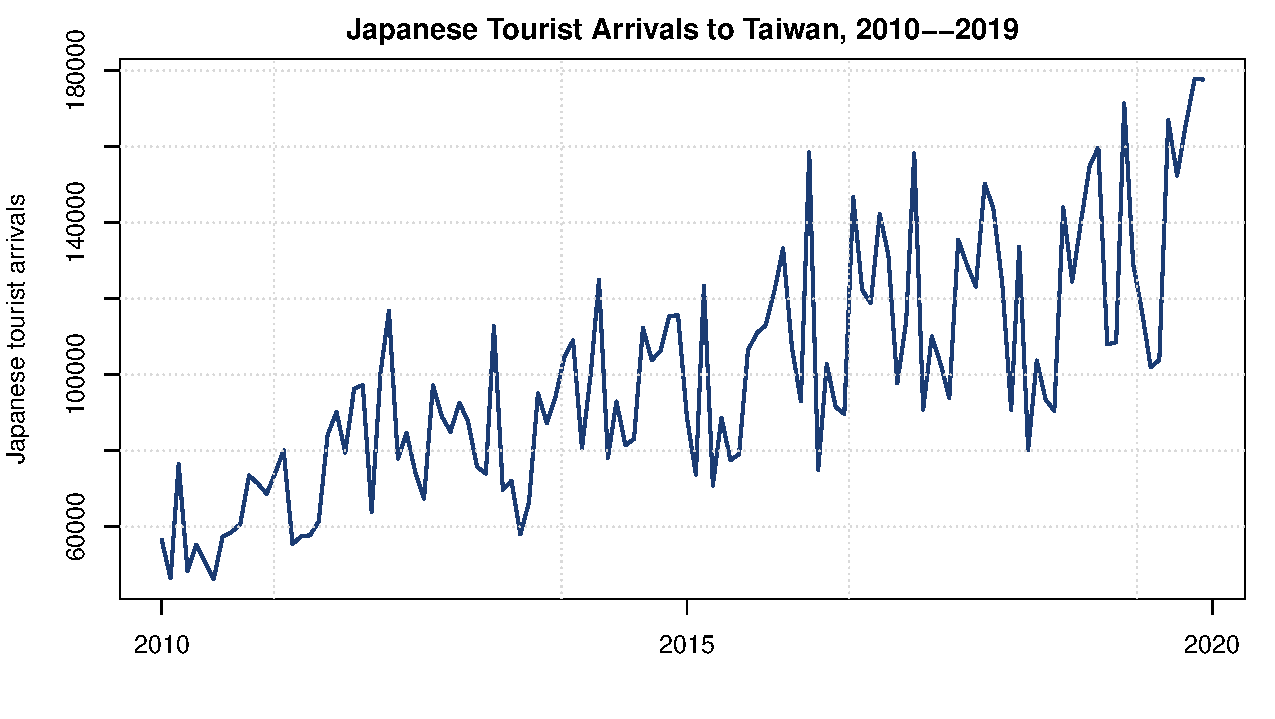
\includegraphics[width=0.84\textwidth]{figures/figure1_tourist_trend.pdf}
\caption{Japanese tourist arrivals to Taiwan, 2010--2019}
\caption*{\footnotesize Note: Graph based on monthly tourist-arrival observations in the project dataset for January 2010 to December 2019.}
\end{figure}

\begin{figure}[H]
\centering
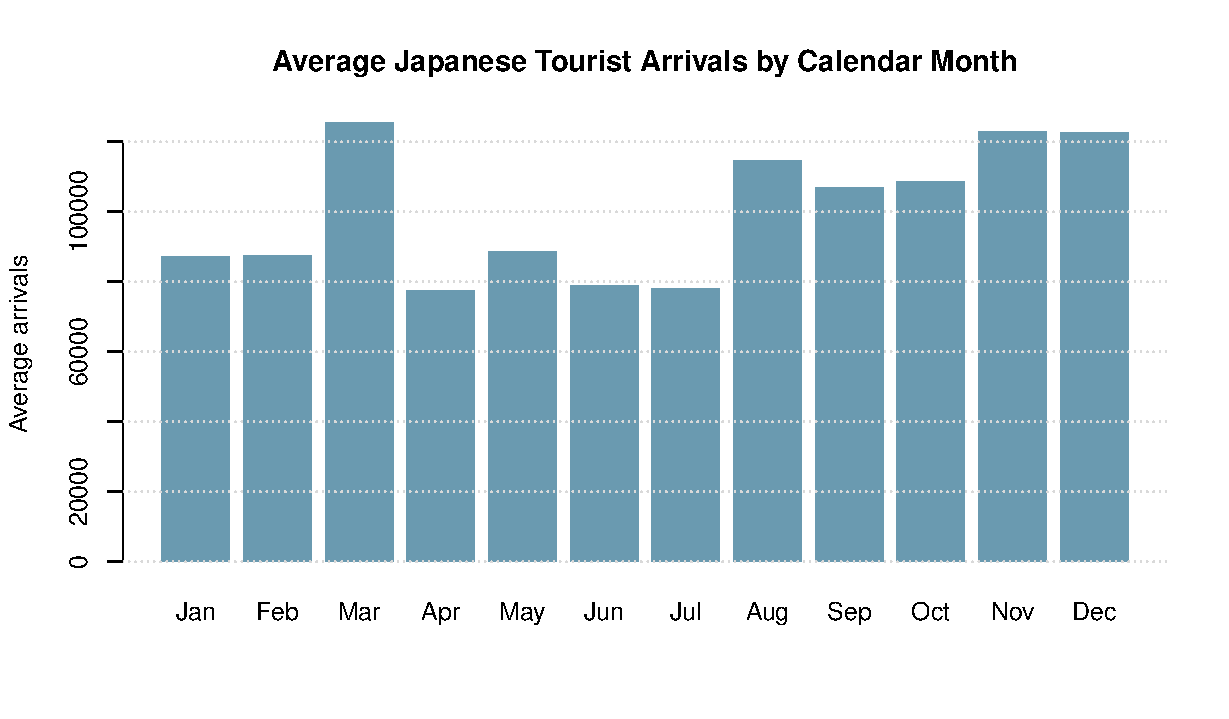
\includegraphics[width=0.78\textwidth]{figures/figure2_seasonality.pdf}
\caption{Average Japanese tourist arrivals by calendar month}
\caption*{\footnotesize Note: Monthly averages are computed from the same sample period. December serves as the high-season reference month in the regressions.}
\end{figure}

Graphs 3 to 5 add descriptive comparisons based on the raw monthly series. To make the movements comparable on one axis, each series is converted into an index with January 2010 set equal to 100. The exchange-rate comparison shows that tourist arrivals and the JPY/TWD index do not move in a simple one-for-one pattern over time, which is consistent with the later finding that the exchange-rate effect is weaker than the trend and seasonal components. The oil-price comparison shows that oil prices fluctuate much more sharply than tourist arrivals, which helps explain why oil-price changes may matter only intermittently rather than as a stable driver of the full series. The industrial-production comparison is useful because it visually tracks the broad co-movement between Japanese economic conditions and tourist arrivals that later appears more clearly in the dynamic model.

\begin{figure}[H]
\centering
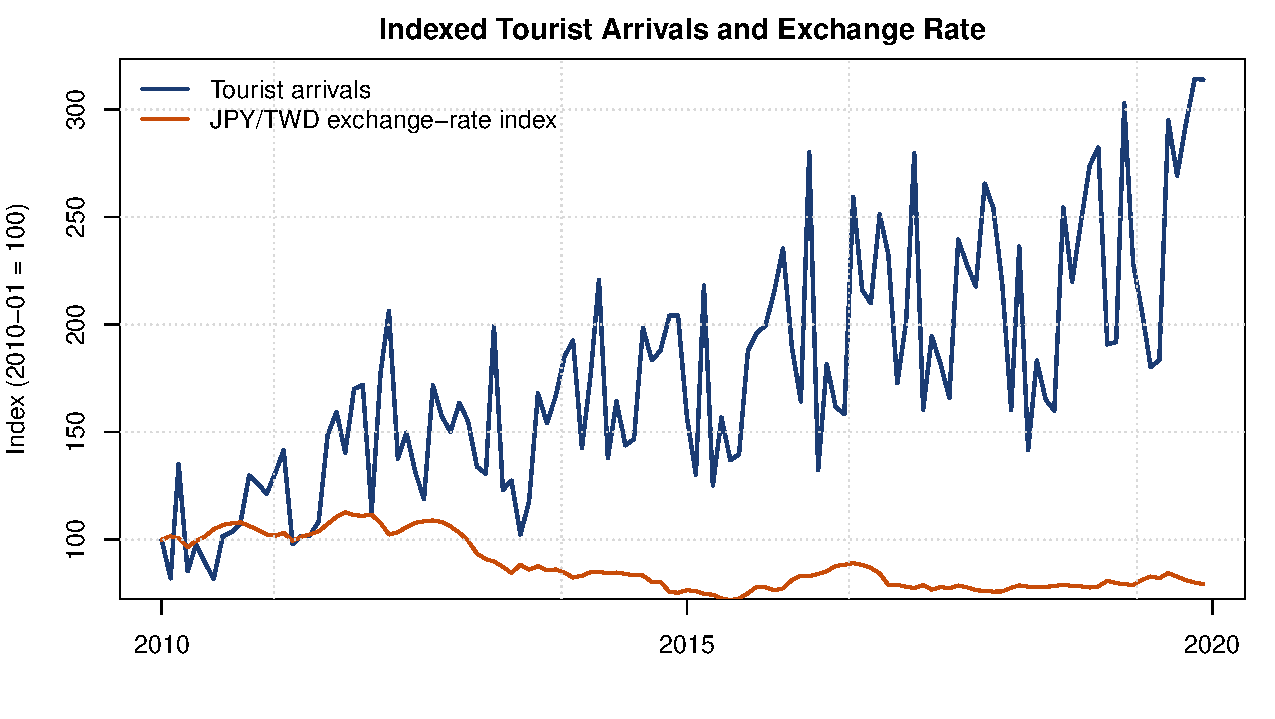
\includegraphics[width=0.84\textwidth]{figures/figure3_tourist_fx_index.pdf}
\caption{Indexed tourist arrivals and the JPY/TWD exchange-rate index (January 2010 = 100)}
\caption*{\footnotesize Note: Both series are rescaled so that January 2010 equals 100. This graph is descriptive and does not impose any regression structure.}
\end{figure}

\begin{figure}[H]
\centering
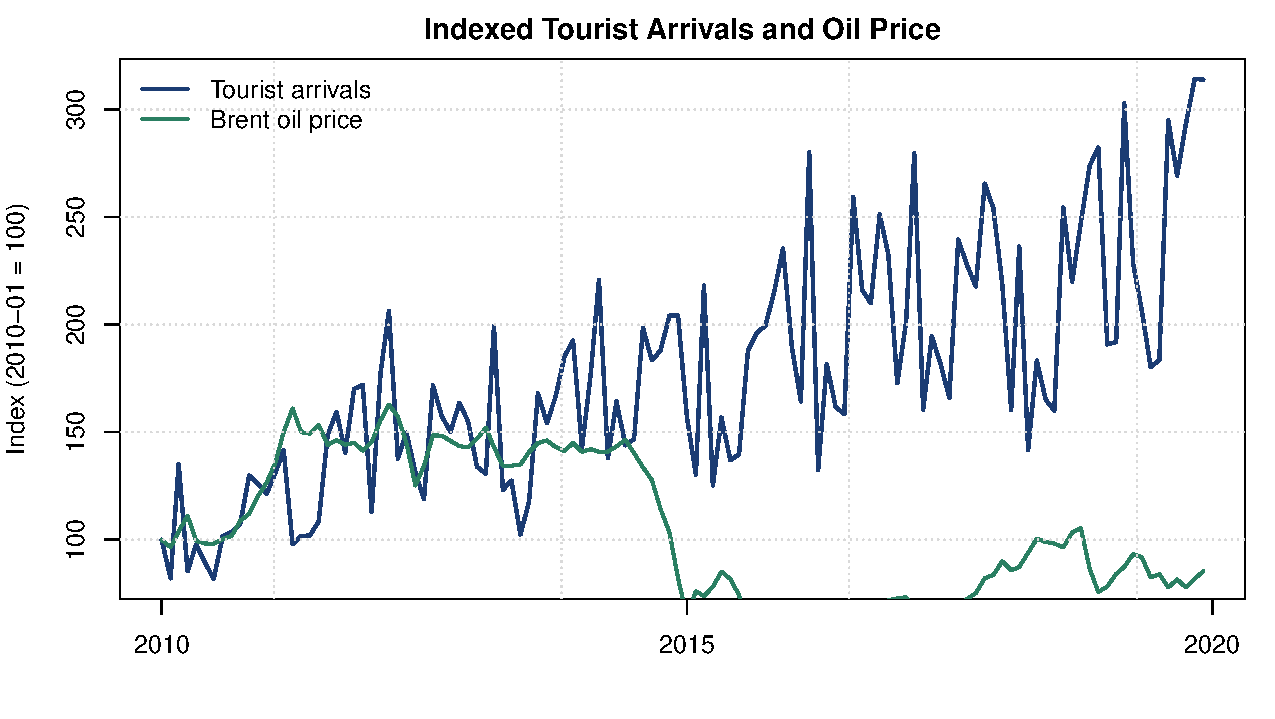
\includegraphics[width=0.84\textwidth]{figures/figure4_tourist_oil_index.pdf}
\caption{Indexed tourist arrivals and Brent oil price (January 2010 = 100)}
\caption*{\footnotesize Note: Both series are rescaled so that January 2010 equals 100. Oil prices show larger short-run swings than tourist arrivals over the sample.}
\end{figure}

\begin{figure}[H]
\centering
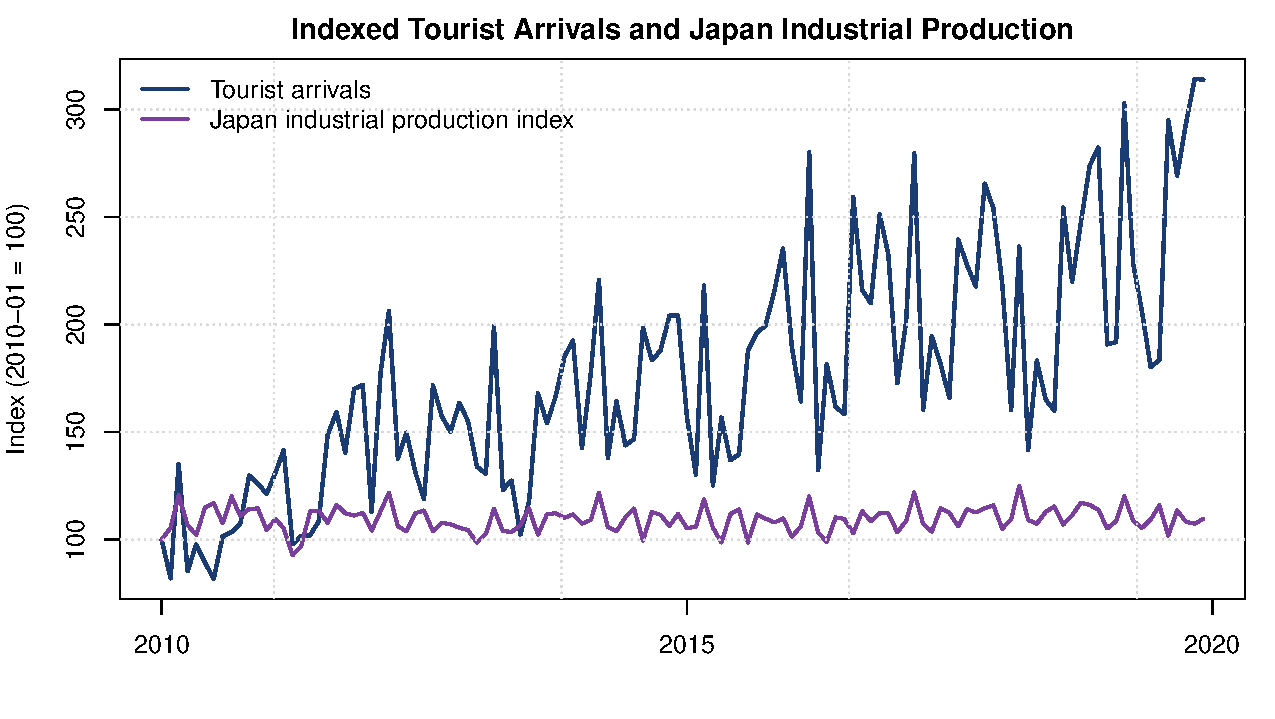
\includegraphics[width=0.84\textwidth]{figures/figure5_tourist_jipi_index.pdf}
\caption{Indexed tourist arrivals and Japan industrial production (January 2010 = 100)}
\caption*{\footnotesize Note: Both series are rescaled so that January 2010 equals 100. The graph highlights broad medium-run co-movement rather than immediate month-to-month responses.}
\end{figure}

\subsection{Main regression results}

\begin{table}[H]
\centering
\caption{Stata-style regression table based on R estimates}
\label{tab:main-results}
\small
\begin{tabular}{lcc}
\toprule
Variable & (1) Static model & (2) Dynamic lag model \\
\midrule
$\Delta \ln(\mathrm{FX}_t)$ & -0.991* & -1.032* \\
 & (0.559) & (0.536) \\
$\Delta \ln(\mathrm{FX}_{t-1})$ & --- & 0.435 \\
 &  & (0.405) \\
$\Delta \ln(\mathrm{FX}_{t-2})$ & --- & -0.098 \\
 &  & (0.392) \\
$\ln(\mathrm{Tourist}_{t-1})$ & --- & 0.505*** \\
 &  & (0.082) \\
$\ln(\mathrm{JIPI}_t)$ & 0.302 & 0.840** \\
 & (0.548) & (0.323) \\
$\ln(\mathrm{JIPI}_{t-1})$ & --- & -0.623* \\
 &  & (0.373) \\
$\ln(\mathrm{JIPI}_{t-2})$ & --- & 0.006 \\
 &  & (0.327) \\
$\Delta \ln(\mathrm{OilPrice}_t)$ & -0.260* & -0.133 \\
 & (0.135) & (0.132) \\
$\Delta \ln(\mathrm{OilPrice}_{t-1})$ & --- & 0.053 \\
 &  & (0.145) \\
$\Delta \ln(\mathrm{OilPrice}_{t-2})$ & --- & 0.116 \\
 &  & (0.129) \\
Time trend & 0.007*** & 0.003*** \\
 & (0.001) & (0.001) \\
Observations & 120 & 120 \\
Adjusted $R^2$ & 0.8805 & 0.9044 \\
HAC standard errors & Yes & Yes \\
\bottomrule
\end{tabular}
\vspace{0.4em}
\begin{minipage}{0.92\textwidth}
\footnotesize
Notes: Newey-West HAC robust standard errors are reported in parentheses. Significance levels are based on HAC p-values. * $p<0.10$, ** $p<0.05$, *** $p<0.01$.
\end{minipage}
\end{table}


In Model 1, the exchange-rate coefficient is \StaticFX{} with a HAC $p$-value of \StaticFXP{}. The coefficient is negative and marginally significant at the 10 percent level. Thus, a one-percentage-point increase in monthly exchange-rate growth is associated with about a 0.991 percent decline in Japanese arrivals. This sign is opposite to the original hypothesis.

Current $\ln(\mathrm{JIPI}_t)$ is positive in Model 1 but not significant. By contrast, $\Delta \ln(\mathrm{OilPrice}_t)$ is \StaticOil{} with a HAC $p$-value of \StaticOilP{}, so higher oil-price growth is associated with lower arrivals and the effect is marginally significant. The time trend is positive and highly significant, indicating strong long-run growth in Japanese arrivals during the sample period.

These findings motivate a comparison with the dynamic specification rather than stopping at the static regression. If part of the unexplained movement in Model 1 reflects persistence in travel demand or delayed macroeconomic transmission, then adding lag structure should both improve fit and clarify which variables remain important once inertia is taken into account.

Model 2 raises the adjusted $R^2$ from \StaticAdjRtwo{} to \DynamicAdjRtwo{}. The lagged dependent variable is \LagTourist{} with a HAC $p$-value of \LagTouristP{}, showing strong persistence in tourist arrivals. The contemporaneous exchange-rate coefficient remains negative, \DynamicFX{}, and remains only marginally significant with HAC $p=\DynamicFXP$. Current $\ln(\mathrm{JIPI}_t)$ becomes positive and significant at the 5 percent level, with coefficient \DynamicJIPI{} and HAC $p=\DynamicJIPIP$. Oil-price terms are not significant in the dynamic specification.

The evidence therefore ranks the main determinants as follows: time trend and seasonality are the most stable factors, lagged arrivals are the clearest dynamic effect, Japanese industrial production matters in the dynamic model, and the exchange-rate effect is weaker and less precisely estimated.

\subsection{Monthly effects}

\begin{table}[H]
\centering
\caption{Monthly dummy coefficients with HAC inference (December as the base month)}
\label{tab:month-effects}
\small
\begin{tabular}{lcccc}
\toprule
Month & Model 1 coef. & Model 1 $p$ & Model 2 coef. & Model 2 $p$ \\
\midrule
January & -0.223*** & $<0.001$ & -0.158*** & 0.001 \\
February & -0.223*** & 0.004 & -0.124* & 0.087 \\
March & 0.089* & 0.080 & 0.164*** & 0.001 \\
April & -0.363*** & $<0.001$ & -0.343*** & $<0.001$ \\
May & -0.225*** & $<0.001$ & -0.017 & 0.760 \\
June & -0.367*** & $<0.001$ & -0.285*** & $<0.001$ \\
July & -0.392*** & $<0.001$ & -0.208*** & $<0.001$ \\
August & 0.006 & 0.927 & 0.271*** & $<0.001$ \\
September & -0.097*** & $<0.001$ & -0.136*** & 0.004 \\
October & -0.093*** & $<0.001$ & -0.020 & 0.662 \\
November & 0.005 & 0.778 & 0.065** & 0.026 \\
\bottomrule
\end{tabular}
\vspace{0.4em}
\begin{minipage}{0.94\textwidth}
\footnotesize
Notes: Coefficients are measured relative to December. HAC/Newey-West p-values are reported. * $p<0.10$, ** $p<0.05$, *** $p<0.01$.
\end{minipage}
\end{table}


The monthly coefficients confirm strong seasonality. In Model 1, March is marginally stronger than December, whereas April, June, and July are significantly weaker. In Model 2, March, August, and November are stronger months relative to December, while April, June, and July remain clearly weaker. These results reinforce the descriptive evidence that seasonal structure is more stable than most macroeconomic coefficients.

\section{Robustness Check}

\begin{table}[H]
\centering
\caption{Diagnostic and robustness checks based on R output}
\label{tab:diagnostics}
\begin{tabular}{lcc}
\toprule
Diagnostic item & Model 1 & Model 2 \\
\midrule
Overall F-statistic & 59.44 & 52.19 \\
F-test p-value & $<0.001$ & $<0.001$ \\
Breusch-Godfrey LM statistic & 27.982 & 16.114 \\
Breusch-Godfrey p-value & $<0.001$ & $<0.001$ \\
Maximum VIF & 3.27 & 9.75 \\
Adjusted $R^2$ & 0.8805 & 0.9044 \\
\bottomrule
\end{tabular}
\end{table}


Both models pass the overall F test at conventional levels, with F statistics of \StaticFstat{} and \DynamicFstat{} and p-values below 0.001. This indicates that each regression is jointly significant as a whole.

At the same time, the Breusch-Godfrey tests remain significant in both models, so residual serial correlation is still present. This is why the paper relies on HAC/Newey-West standard errors rather than conventional OLS inference. Model 2 reduces the BG statistic relative to Model 1, but it does not remove the problem entirely.

The VIF results show that multicollinearity is limited in Model 1, where the maximum VIF is \MaxVIFStatic{}, but more concerning in Model 2, where it rises to \MaxVIFDynamic{}. This does not invalidate the model, but it cautions against strong interpretation of individual lag coefficients, especially the lagged industrial-production terms.

Graph 6 compares actual and fitted values. The dynamic model tracks the series more closely than the static model, but the remaining unexplained short-run movement supports a cautious reading of the exchange-rate coefficient.

\begin{figure}[H]
\centering
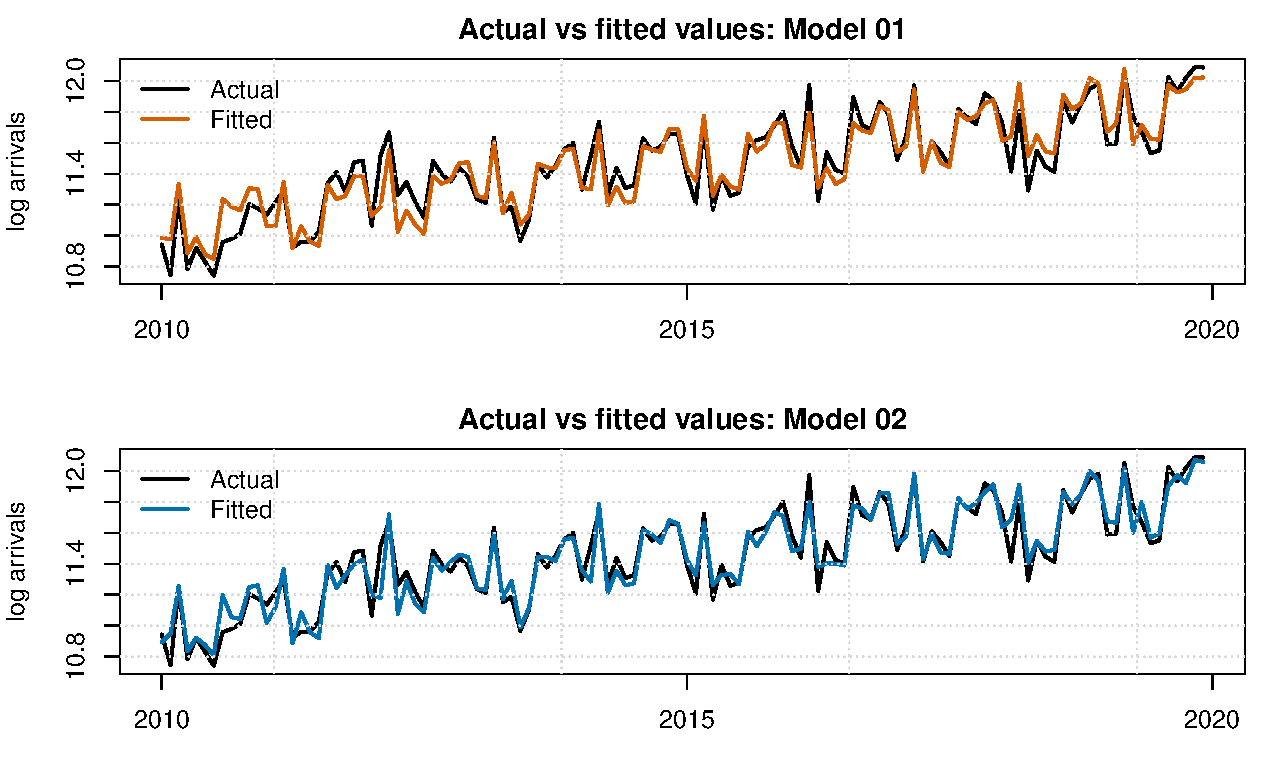
\includegraphics[width=0.86\textwidth]{figures/figure6_actual_vs_fitted.pdf}
\caption{Actual and fitted values from Model 1 and Model 2}
\caption*{\footnotesize Note: Fitted values are produced from the two estimated models and are shown here only to compare overall tracking performance.}
\end{figure}

\section{Limitations and Unresolved Issues}

The results should be read with several limitations in mind. First, the empirical design is intentionally restricted to 2010--2019 in order to avoid the extraordinary disruption created by the COVID-19 period. That choice is reasonable for isolating pre-pandemic tourism behavior, but it also means that the estimated trend reflects a relatively normal decade and should not be extrapolated mechanically to later periods. In addition, although the estimation window begins in January 2010, the global financial crisis of 2008--2009 may still have had lagged effects on income expectations, travel confidence, and outbound tourism behavior in the early part of the sample. The paper does not model those lingering post-crisis effects separately.

Second, the specification focuses on a limited set of macroeconomic regressors. The exchange rate, industrial production, oil prices, trend, and month dummies capture some important channels, but they do not exhaust the determinants of Japanese travel demand. In particular, the analysis does not separately control for natural disasters, aviation capacity, airfare movements, destination-specific promotion, competing destination prices, or bilateral policy changes. This omission matters because shocks such as typhoons, earthquakes, or Japanese trade and tariff policy changes may affect both tourism behavior and broader financial conditions, including exchange-rate movements. Without an identification strategy that isolates exogenous exchange-rate variation, the estimated exchange-rate coefficient should be interpreted as an association rather than a clean causal effect.

Third, the time-series treatment is practical rather than fully comprehensive. Because ADF results indicate non-stationarity in $\ln(\mathrm{FX}_t)$ and $\ln(\mathrm{OilPrice}_t)$, the paper uses first differences for those variables, which means the regressions mainly capture short-run effects. The current framework therefore does not recover a long-run exchange-rate elasticity. A richer approach such as an ARDL or error-correction framework could be considered in future work if the goal were to distinguish more systematically between short-run and long-run relationships.

Fourth, the dynamic specification improves fit but does not solve every econometric concern. Model 2 is motivated by both tourism-demand persistence and the residual serial correlation detected after the static model. However, the choice of two lags is a practical modeling decision rather than the outcome of a formal lag-selection exercise based on AIC or BIC. Moreover, the Breusch-Godfrey tests remain significant even after lags are added, so HAC/Newey-West corrections improve inference but do not eliminate all dynamic misspecification. The higher VIF values in Model 2 also caution against strong interpretation of individual lag coefficients, especially when their signs are unstable.

These limitations are important for interpreting the negative exchange-rate coefficient. The result is informative, but it should not be overstated. It may reflect destination substitution, safe-haven movements in the yen, omitted shocks, or timing frictions in travel planning. The present paper identifies that pattern in the data, but it does not fully resolve which mechanism dominates.

\section{Conclusion}

This paper finds that the JPY/TWD exchange-rate coefficient is negative in both the static and dynamic specifications, contrary to the original expectation that yen appreciation should raise Japanese tourist arrivals to Taiwan. However, this exchange-rate effect is only marginally significant under HAC inference and should therefore be interpreted cautiously. By contrast, time trend, seasonal effects, and lagged tourist arrivals are more stable and more precisely estimated determinants.

The results therefore support a restrained conclusion rather than a strong causal claim. Yen appreciation may coincide with destination substitution, safe-haven behavior in foreign-exchange markets, or other macro-financial conditions rather than a simple bilateral price effect. Moreover, unresolved issues such as omitted disaster shocks, possible lingering post-crisis effects, residual serial correlation, and the absence of an instrumental-variable strategy limit how far the exchange-rate coefficient can be pushed in policy interpretation.

The practical implication is not that exchange rates are irrelevant, but that they are unlikely to be the dominant margin through which Taiwan can influence Japanese arrivals in the short run. The evidence in this paper suggests that seasonal structure, persistence in tourism demand, and broader market competitiveness matter more consistently than month-to-month exchange-rate movements. Future work should therefore examine richer event controls, alternative lag structures, and stronger identification strategies before drawing firmer conclusions about the causal role of the JPY/TWD exchange rate.

\begin{thebibliography}{99}

\bibitem[Lim(1997)]{lim1997}
Lim, C. (1997).
Review of international tourism demand models.
\textit{Annals of Tourism Research}, 24(4), 835--849.

\bibitem[Seetaram et~al.(2016)Seetaram, Forsyth, and Dwyer]{seetaram2016}
Seetaram, N., Forsyth, P., \& Dwyer, L. (2016).
Measuring price elasticities of demand for outbound tourism using competitiveness indices.
\textit{Annals of Tourism Research}, 56(1), 65--79.

\bibitem[Song and Li(2008)]{songli2008}
Song, H., \& Li, G. (2008).
Tourism demand modelling and forecasting: A review of recent research.
\textit{Tourism Management}, 29(2), 203--220.

\end{thebibliography}

\section*{Data Sources}

\begingroup
\sloppy
\begin{itemize}
\item Tourism Administration, Republic of China (Taiwan): Japanese tourist arrivals to Taiwan. \url{https://stat.taiwan.net.tw/inboundSearch}
\item Central Bank of the Republic of China (Taiwan): JPY/TWD exchange rate. \url{https://cpx.cbc.gov.tw/Range/RangeSelect?pxfilename=BP01M01.px}
\item Federal Reserve Bank of St. Louis, FRED series POILBREUSDM: Brent crude oil price. \url{https://fred.stlouisfed.org/series/POILBREUSDM}
\item Federal Reserve Bank of St. Louis, FRED series JPNPRINTO01IXOBM: Japan industrial production index. \url{https://fred.stlouisfed.org/series/JPNPRINTO01IXOBM}
\end{itemize}
\endgroup

\end{document}
